%\usepackage{hyperref}

%\section{Systematic uncertainties For \HwwZqq\}
\section{Systematic uncertainties }
\label{sec:systematics}

%as follows:
%\begin{itemize}
%\item Background-related systematic uncertainties: background parametrization.
%\item Signal-related systematics uncertainties: H-tagging efficiency, b-tagging scale factor, PDF uncertainties, 
The sources of systematic uncertainties are summarized here:  
:H-tagging efficiency, b-tagging scale factor, PDF uncertainties, 
W/Z-tagging efficiency, Jet Energy Scale(JES), Jet Energy Resolution(JER), luminosity, cross-talk of various signals.
%\end{itemize}


%\subsection{Background shape parametrization}
%\label{sec:background}
%We search for a peak on top of the falling background spectrum by
%means of a maximum likelihood fit to the data. The fit parameters have 
%flat priors and are left freely floating during the Signal+Background fit. 
%The uncertainty from S+B background fit is taken into account in limit setting
%by    
%The background uncertainty is taken into

%account by profiling out the background fit parameters

\subsection{b-tagging scale factor}
We use method 1c recommended by the BTV group to apply b-tagging scale factor and uncertainties, 
which is \url{https://twiki.cern.ch/twiki/bin/viewauth/CMS/BTagSFMethods\#1c\_Event\_reweighting\_using\_scale}. 

if $\Delta R$ of the two subjets is bigger 
than 0.3, we apply the b-tagging scale factor
on the two subjets. While $\Delta R$ is between 0.3 to 0.4,  
we double the b-tagging scale factor uncertainties.
When $\Delta R$ is smaller than 0.3, we apply the 
b-tagging scale factor on the fat jet.
The uncertainty from b-taggging scale factor is evaluated by taking the largest difference 
in tagging efficiency by shifting
 b-tagging scale factor 1 $\sigma$, which results in 15\% uncertainty. 

\subsection{W/Z-tagging efficiency}
\label{sec:vtageff}

W/Z-tagging efficiency scale factor is studied in hadronic
 VV search~\cite{CMS:2013fea, JME-13-006}, details following.
%We follow the same procedure as described in Ref.~\cite{JME-13-006} , described below.
%Quoted from {\bf EXO-12-024}. 
The W/Z-tagging efficiency is determined from the Monte Carlo simulation.
We cross-check the MC modelling of the signal efficiency by measuring the W/Z-tagging efficiency
in semileptonic $\ttbar$ data, and compare it
with the same efficiency obtained using identical 
procedure from $\ttbar$ Monte Carlo sample generated 
with MadGraph~\cite{madgraph} and showered with Pythia6 Tune Z2*.
The ratio of the two efficiencies defines a scale factor, which is then applied to
the efficiencies for signals in the dijet data.

%The efficiency of the cut on the $\tau_{21}$ variable in the semileptonic $\ttbar$ sample is found to be \mucuteffsemilepdata for data, %and \mucuteffsemilepmc for Monte Carlo.
%The efficiency of the pruned jet mass cut for the data and Monte Carlo are \mcuteffsemilepdata and \mcuteffsemilepmc, respectively.
Combining the efficiencies of the $\tau_{21}$ and jet mass cuts,
 a data-MC scale factor of  \scalefactorHP
(\scalefactorLP) for the high (low) purity selection for the  W-tagging efficiency is determined.
We assume that the same scale factor applies to Z-tagging as well.
The errors on the scale factor are propagated
into the systematic uncertainties on the overal signal efficiency.


%\begin{figure}[htb]
%\centering
%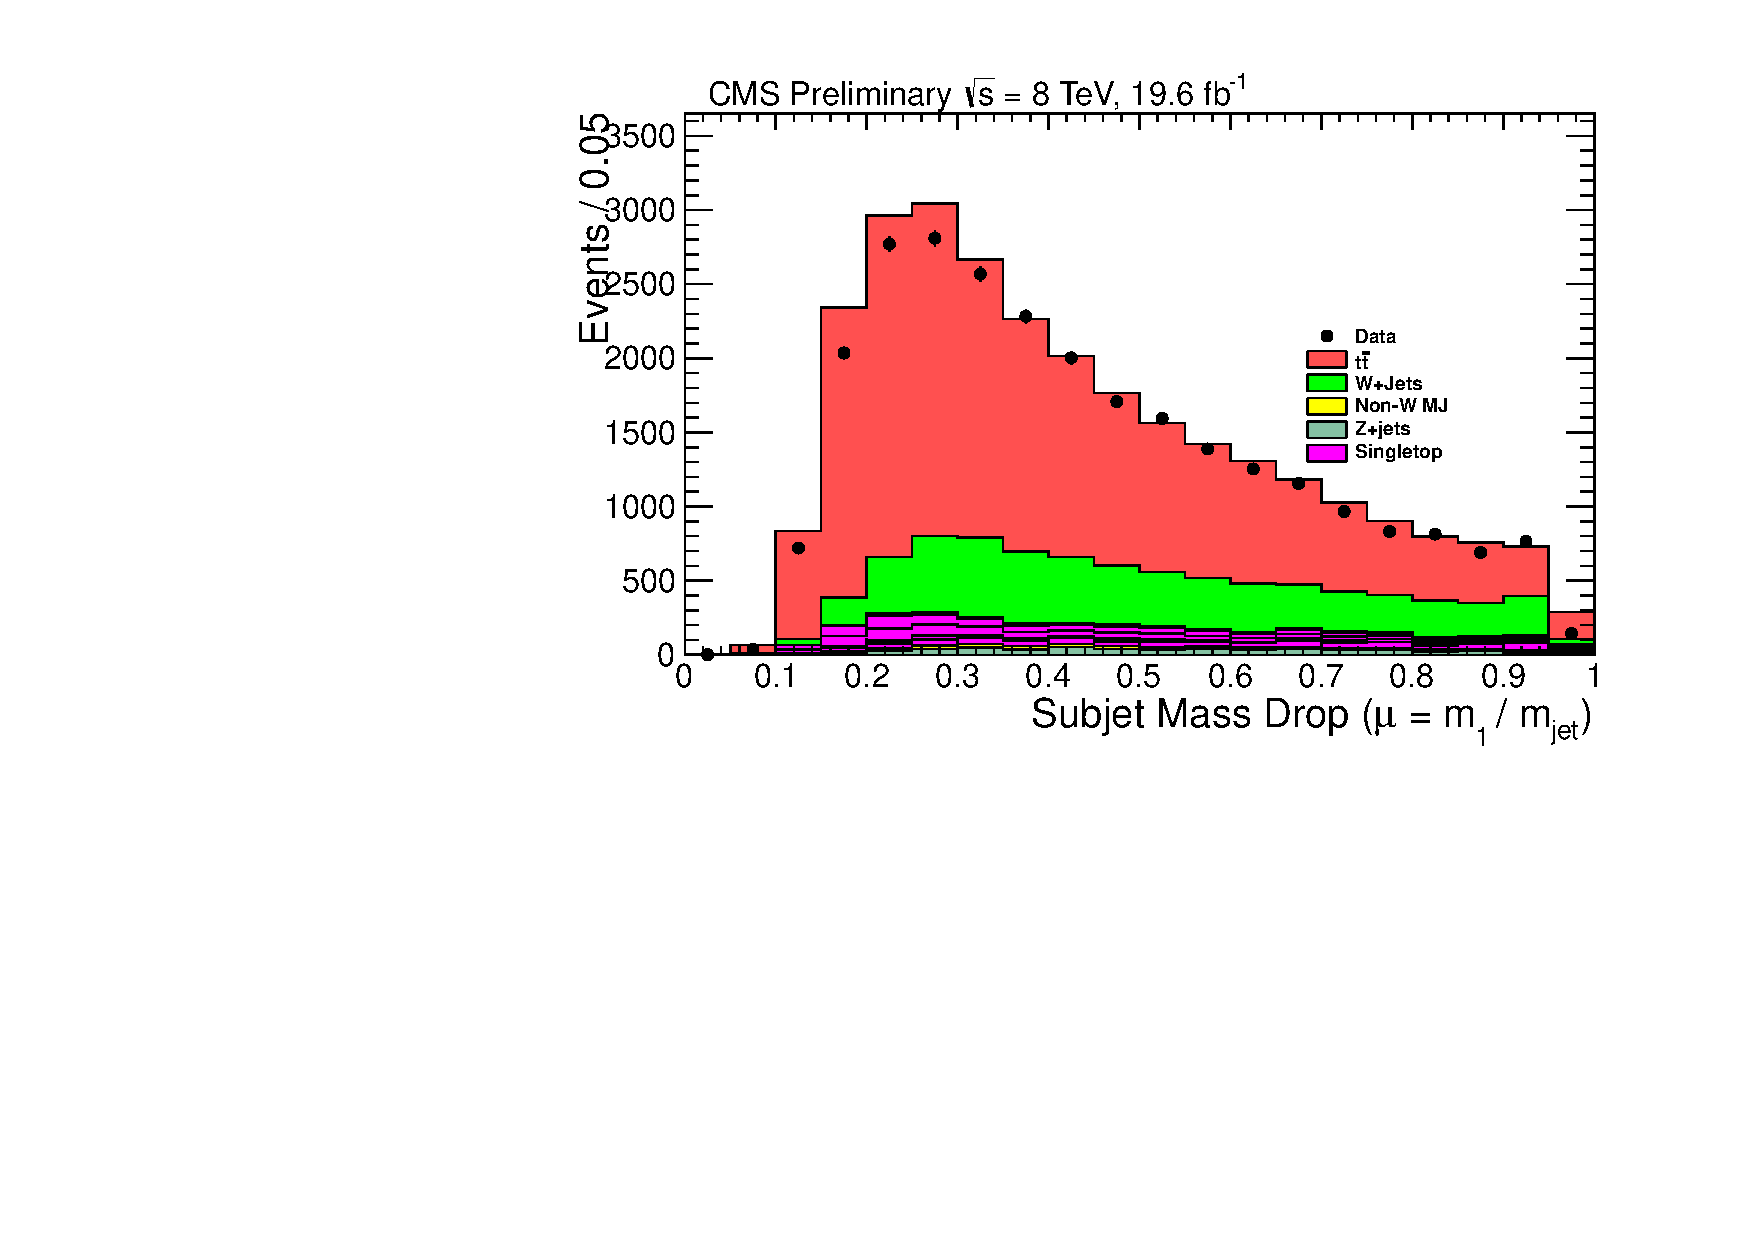
\includegraphics[width=0.95\textwidth]{figs/semiLepMass_muHist}
%\caption{$\tau_{21}$ of the highest mass jet in a semileptonic
%ttbar sample from Ref.~\cite{hadronictop}.}
%\label{figs:muHist_semileptonic}
%\end{figure}

%\begin{figure}[htbp]
%\centering
%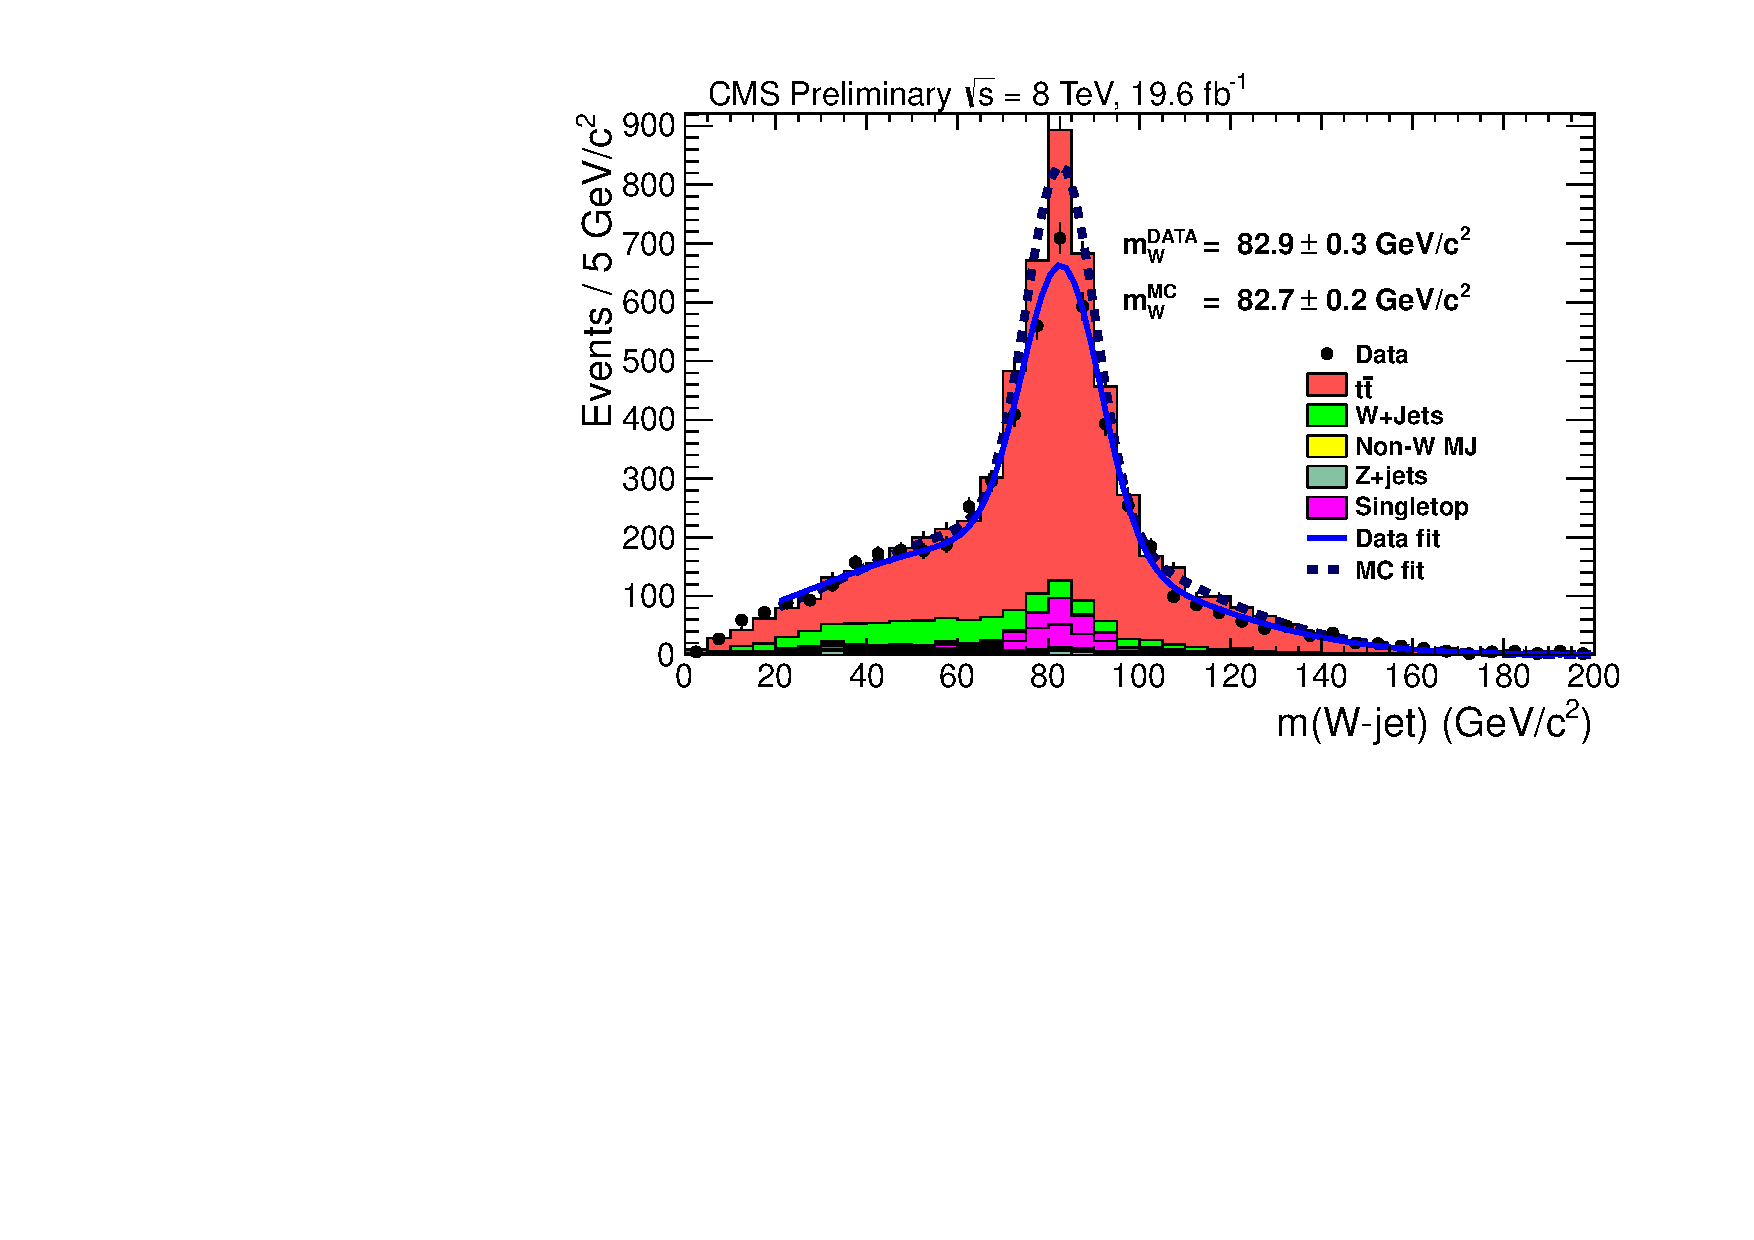
\includegraphics[width=0.95\textwidth]{figs/semiLepMass_mWCand.pdf}
%\caption{Pruned jet mass of the highest mass jet in a semileptonic
%ttbar sample from Ref.~\cite{hadronictop}.}
%\label{figs:mHist_semileptonic}
%\end{figure}


The efficiency error on a single $\PW/\cPZ$-tagging is estimated with
a control sample of semileptonic $t \bar t$ events as described above.
The uncertainties of \scalefactorHPu (\scalefactorLPu) on the scale
factors for high (low) purity tagging include sources from control
sample statistics, pruned jet mass scale and pruned jet mass
resolution.
Since we estimate the scale factor
only in the kinematic regime of the $\ttbar$ sample where the W decay
products merge, but the b-quarks are still reconstructed as separate
jets, we need to rely on the simulation to extrapolate to
higher jet \pt.


Therefore, we estimate how the W/Z jets tagging efficiency varies 
as a function of
\pt for two different showering and hadronization models using
\PYTHIA~6 and \HERWIG{++}.
We find that the differences are within $4\%$ ($12\%$)
for the high (low) purity tagging~\cite{CMS:2013fea}, 
significantly smaller than the statistical uncertainties in the scale factors.
%, the results are summarized in 
%Table~\ref{table:Difference}.  
% and therefore smaller than the
%statistical uncertainty of the scale factor.


%\GBulk samples generated with {\sc jhugen} and interfaced with
%\PYTHIA~6 and \HERWIG{++}.
%Also, the dijet mass dependence of the $\PW/\cPZ$-tagging efficiency for
%background events, shown in Fig.~\ref{fig:singleefficiencies} and Fig.~\ref{fig:doubleefficiencies},
%is adequately described by the simulation.
\subsection{H-tagging efficiency for $\Hww$ tagger}

We extrapolate the H-tagging efficiency scale factor 
from the W/Z-tagging efficiency scale factor, more details are 
in Appendix~\ref{tau42SF}.
In $\Hww$, Higgs will decay to one on-shell W and one off-shell W. The 
on-shell W decays similarly as a single W/Z jet.
 while the off-shell W, is soft. 
So the overall Higgs
jet could be viewed as a real W/Z jet plus soft part.    
To the first order approximation, 
we apply the same scale factor to H-tagging as W/Z-tagging, but 
with an additional uncertainty.


For W/Z tagging, which uses $\tau_{21}$, we know exactly 
the scale factor at low pt and need no additional uncertainty 
from Pythia/Herwig. So the Herwig efficiency as a function
 of pT can be normalized in such a way
 that Pythia and Herwig agree at low pT, 
but are different at high pT.

For $\tau_{42}$ we don't know if it is correct at low pT and
high pT. Therefore, we should be more conservative 
and take the Pythia-Herwig difference
 without normalizing them at low pT. 

%The effects of the transition from $\tau_{21}$ to $\tau_{42}$ is 
%evaluated from generator differences. 
We estimate how the Higgs jet tagging efficiency varies
as a function of
\pt for two different showering and hadronization models using
\PYTHIA~6 and \HERWIG{++}.
We find that the differences are within $7\%$ ($7\%$)
for the high (low) purity tagging, the results are summarized in
Table~\ref{table:Difference}.

\begin{table}[htbp]
\begin{center}
\caption{
The difference of $\Hww$ jet tagging efficiency in signal MC 
by showering and hadronization with Pythia and Herwig. Higgs jets
are the jets matched to Higgs generator particles. } 
\label{table:Difference}

\begin{tabular}{|l|r|r|r|r|}
\hline
Resonance & \multicolumn{1}{l|}{1000GeV} & \multicolumn{1}{l|}{1500GeV} & \multicolumn{1}{l|}{2000GeV} & \multicolumn{1}{l|}{2500GeV} \\ 
High Purity Higgs jets & 4.75\% & 2.28\% & 1.52\% & 6.31\% \\ 
Low Purity Higgs jets & 5.91\% & 6.33\% & 0.79\% & 4.39\% \\ \hline
%High Purity Z gen & 9.80\% & 7.58\% & 6.82\% & 6.98\% \\ \hline
%Low Purity Z gen & 15.44\% & 13.03\% & 10.18\% & 8.83\% \\ \hline
%Dijet Mass High Purity & 13.09\% & 8.67\% & 8.74\% & 4.71\% \\ \hline
%Dijet Mass Low H & 16.77\% & 17.34\% & 2.53\% & 8.94\% \\ \hline
%Dijet Mass LowV & 15.52\% & 8.99\% & 8.00\% & 8.72\% \\ \hline
\end{tabular}
\end{center}
%The difference of \HwwZqq\ signal in tagging efficiency
% by showering and 
%hadronization with pythia and herwig. Higgs gen and Z gen are the gen jets 
%that are matching to the Higgs and Z generator particles. }
\end{table}


\subsection{Other uncertainties}

%Other systematic errors on the tagging efficiency are small or
%negligible.
Because of the rejection of charged particles not
originating from the primary vertex and also the application of
pruning, the pileup dependence on the $H/\PW/\cPZ$-tagging efficiency
is weak, and the uncertainty of the modeling of the pileup
distribution is less than 3\%.  Modeling of the underlying event,
estimated by switching it off in \PYTHIA~6, and also by comparing 
different tunes of \PYTHIA~6, 
impacts the tagging
efficiency by less than 1\%. %  These
%systematic errors refer to a single $\PW/\cPZ$-tagged jet and are
%applied twice for double $\PW/\cPZ$-tagged events.

In the jet \PT and $\eta$ regions considered in this analysis,
the Jet Energy Scale is known to a precision of 1-2\%~\cite{JME-JINST,Collaboration:2013dp}.
For JES, \PT and $\eta$ dependent uncertainty is
propagated to the reconstructed dijet invariant mass,
and taken into account by shifting the resonance dijet mass
 in the statistical analysis.

The Jet Energy Resolution(JER) is known
to a precision of 10\% and its tails are in
agreement between data and MC~\cite{JME-JINST}.
The JER is taken into account in the statistical analysis
 by a variation of the resonance width by 10\%.  
%We estimate the JES and JER impacts on the tagging efficiency by shifting them
% 1 $\sigma$ respectively,
% and taking the largest variation in tagging efficiency as uncertainty, which 
%is 12\% from JES and 4\% from JER.  


The JES and JER of b jets are studied by JETMet, showing a 
smaller uncertainty than the standard QCD mixture of light quarks and gluon jets, whose JES and JER are applied 
for all flavor jets in this analysis. 
So we don't 
apply additional specific JES and JER uncertainty for b jets. 
%We evaluate the effects of JES and JER on the pruned jet mass cut we 
%applied by selecting Higgs and V jets by 
%We apply a gaussian plus crystal-ball function fit 
%on the reconstructed signal resonance mass distribution.
%By shifting the fit paramter 1 $\sigma$,    
The uncertainty on the pruned jet mass cut of $\Hww$ is included in the scale factor extrapolated
from W-tagging. For $\Hbb$ tagger, pruned jet mass uncertainty is evaluated as 2.6\%, synchronized with
EXO-12-053.  

The uncertainty related to the PDF used to model the signal acceptance is estimated
from the eigenvectors of the CT10, MRST2008 and NNPDF sets of PDF. The 
envelope of the upward and downward variations of the estimated acceptance of the three
 sets is assigned as uncertainty and found to be 5\%-15\% in the resonance mass range of 
interest.    

The luminosity has been measured with 
an uncertainty of 2.6\%~\cite{LUM-13-001}, 
and is also taken into account in the statistical analysis.

For the cross-talk of Higgs signals, we assign them as systematic uncertainty. 
In this analysis, signals are generated in exclusive decay channels, for example, \HbbVqq signals only have 
$\Hbb$ decays, no other Higgs decays. 
So in category Hbb1 and Hbb2,  the only signal is \HbbVqq, other Higgs decays passing the $\Hbb$ tagger will 
be assigned as systematic uncertainties, which is evaluated according to Equation~\ref{eq:uncer}. 
\begin{equation}
%Uncertainty_{Cross-talk} = \frac{NumberofExpectedNuisanceSignals}{NumberofCorrespondingData}  
Uncertainty_{Cross-talk} = \frac{\#TotalExpectedSignals}{\#SignalOfInterest} - 1 
%P_D(m_\mathrm{jj}) = \frac{P_{0} (1 - m_\mathrm{jj}/\sqrt{s})^{P_{1}}}{(m_\mathrm{jj}/\sqrt{s})^{P_{2}}} \ .
\label{eq:uncer}
\end{equation}
\noindent For $\Hbb$ tagger, signal of interest is $\Hbb$ signals. All other Higgs decays are taken as nuisance signals.
For $\Hww$ tagger,  signal of interest would be $\Hbb$ plus $\Hww$ and all other Higgs decays are taken as 
nuisance signals.  This number is evaluated across various resonance signal masses, resulting in 7\% for category Hbb1
and Hbb2. This uncertainty is 31\% for Hww1, Hww2 and Hww3, including 9.4\% uncertainty from $\Hzz$ decays, and 21\% from 
Hcc,Hgg, etc.  ${\rm H \to ZZ}$ is taken as having the same efficiency as $\Hww$, as discussed in Table~\ref{table:HbbHww}.   
%,and less than 1\% for category Hbb2.   
%For categories Hww1, this results in 3\% uncertainty, and less than 1\% for Hww2 and Hww3.    

%\noindent As shown in Table~\ref{table:HbbHww},  is 6\% at 2 TeV, 4\% at 1.5 TeV.
%Considering Figure~\ref{fig:HbbZqqBG}, in category Hbb1, 
%the expected $\HbbVqq$ signals around 1.5-2.0 TeV could be comparable to data.
%And in this resonance mass region, nuisance Higgs decays are at most 6\% of $\Hbb$ decays.  
%So we assign 6\% as the cross-talk uncertainty for category Hbb1.
%For Hbb1,   
%For Hww1, Hww2 and  Hww3 categories, although other Higgs decays channel could
%be count around 30\% of the $\Hww$ channels. However, their expected contamination in data, 
%is tiny, which could be validated from Figure~\ref{fig:HwwZqqBG}, where the expected signal of \HwwVqq 
%is already around 5\% of data.  

%As we stated in previous section, the possibility for other Higgs signals, except 
%$\Hbb$ channels, to pass $\Hbb$ tagger, is at most 7\%. 
%And the possibility for other Higgs
%signals, to pass $\Hww$ tagger, is at most 25\% of Hww plus Hbb signals.
%So the other Higgs signals' contribution in the data, is negligible, as we could tell from 
%Figure~\ref{fig:HbbZqqBG} and Figure~\ref{fig:HwwZqqBG}, where the expected ratio of Hbb and Hww signal
%is small compared to data.
%Since we generate our signals in exclusive decay modes of Hbb and Hww, and also because 
%other signals' contribution are small enough, we don't specifically study other Higgs signals, but 
%assign them as systematic uncertainties. We evualuate this uncertainty of these Higgs decays modes 
%by varying its branching ratio 1 $\sigma$ and compare the change on the fraction of these Higgs decay modes to 
%pass $\Hww$ and $\Hbb$ tagger with respect to Hww and Hbb signals. 
%This results in an uncertainty less than 1\%. 

%For the uncertainty from cross-talk, we assign an systematic uncertainty 
%as the ratio, which is  number\_of\_other\_Higgs\_decays\_passing\_tagger / number\_of\_total\_Higgs\_decays\_pass\_tagger. 
%Based on Table~\ref{table:HbbHww}, for categories Hbb1, Hbb2, we assign 6\% uncertainty. For \HwwVqq signals in categories Hww1, Hww2, Hww3, 
%we assign 25\% uncertainty. For \HbbVqq signals in Hww1, Hww2, Hww3 categories, we assign 45\% uncertainty. 

Table~\ref{table:systematicsAll} shows a summarization of all the systematics applied. 


\begin{sidewaystable}[htbp]
\caption{Summarization of systematics.Numbers in parenthesis are for low purity categories.}
\begin{tabular}{|l|l|l|l|l|}
\hline
Systematics/Signals  &  Relevant quantity &
\multicolumn{2}{c|}{\HbbVqq} & \multicolumn{1}{l|}{\HwwVqq} \\ \hline
% & & Pass $\Hbb$ tagger & \multicolumn{1}{l|}{Fail $\Hbb$ tagger, but}    & \multicolumn{1}{l|}{Fail $\Hbb$ tagger, but} \\ 
 & & Hbb1, Hbb2 &  Hww1, Hww2, Hww3   & Hww1,Hww2,Hww3 \\ \hline 
% & &  & pass $\Hww$ tagger & \multicolumn{1}{l|}{pass $\Hww$ tagger} \\ \hline
% & &  & pass $\Hww$ tagger & \multicolumn{1}{l|}{pass $\Hww$ tagger} \\ \hline
 
Background fit  & Resonance shape & \multicolumn{1}{l|}{shape} & \multicolumn{1}{l|}{shape} & \multicolumn{1}{l|}{shape} \\ %\hline
Integrated Luminosity & Yield (per event) &2.6\% & 2.6\% & 2.6\% \\ %\hline
cross-talk            & Yield (per event) &7.0\% & 31\%  & 31\% \\
%JES impacts on tagging efficiency & Yield (per event) & 12.0\% & 12.0\% & 12.0\% \\ %\hline
%JER impacts on tagging efficinecy & Yield (per event) &4.0\% & 4.0\% & 4.0\% \\ %\hline
Dijet mass shift due to JES & Resonance shape & 1.0\% & 1.0\%   & 1.0\% \\
Dijet mass shift due to JER & Resoancne shape & 10.0\%  &  10.0\%  & 10.0\%  \\
PileUp &Efficiency (per jet) & 1.5\% & 1.5\% & 1.5\% \\ %\hline
PDF & Yield (per event) &5-15.0\% & 5-15.0\% & 5-15.0\% \\ %\hline
B-tagging SF & Yield (per event) & 15.0\% & 1.0\% & 15.0\% \\ %\hline
Higgs mass  & Efficiency (per jet) & 2.6\% & 2.6\% & - \\
W-tagging \pt dependence  & Efficiency (per jet)& \multicolumn{1}{l|}{7.5\%(54\%)} & \multicolumn{1}{l|}{7.5\%(54\%)} & \multicolumn{1}{l|}{7.5\%(54\%)} \\ %\hline
W-tagging $\tau_{21}$ extrapolation & Efficiency (per jet) & 4\%(12\%) & 4\%(12\%)  & 4\%(12\%) \\
%tau21 shower/hadronization  & \multicolumn{1}{r|}{4\%(12\%)} & \multicolumn{1}{r|}{4\%(12\%)} & \multicolumn{1}{r|}{4\%(12\%)} \\ %\hline
H-tagging $\tau_{42}$ & Efficiency (per jet)  & \multicolumn{1}{l|}{-} & \multicolumn{1}{l|}{7.5\%(54\%)} & \multicolumn{1}{l|}{7.5\%(54\%)} \\ %\hline
H-tagging $\tau_{42}$ extrapolation & Efficiency (per jet) & \multicolumn{1}{l|}{-} & \multicolumn{1}{l|}{7\%(7\%)} & \multicolumn{1}{l|}{7\%(7\%)} \\ \hline
\end{tabular}
\label{table:systematicsAll}
\end{sidewaystable}


\clearpage
